\chapter{Link--Discovery--Framework}

\section{Modell des Weltausschnittes}
\label{world_model}

Der folgende Abschnitt beschäftigt sich mit der Modellierung des im Rahmen dieser Arbeit verwendeten Weltausschnittes. 

\begin{figure}
\centering
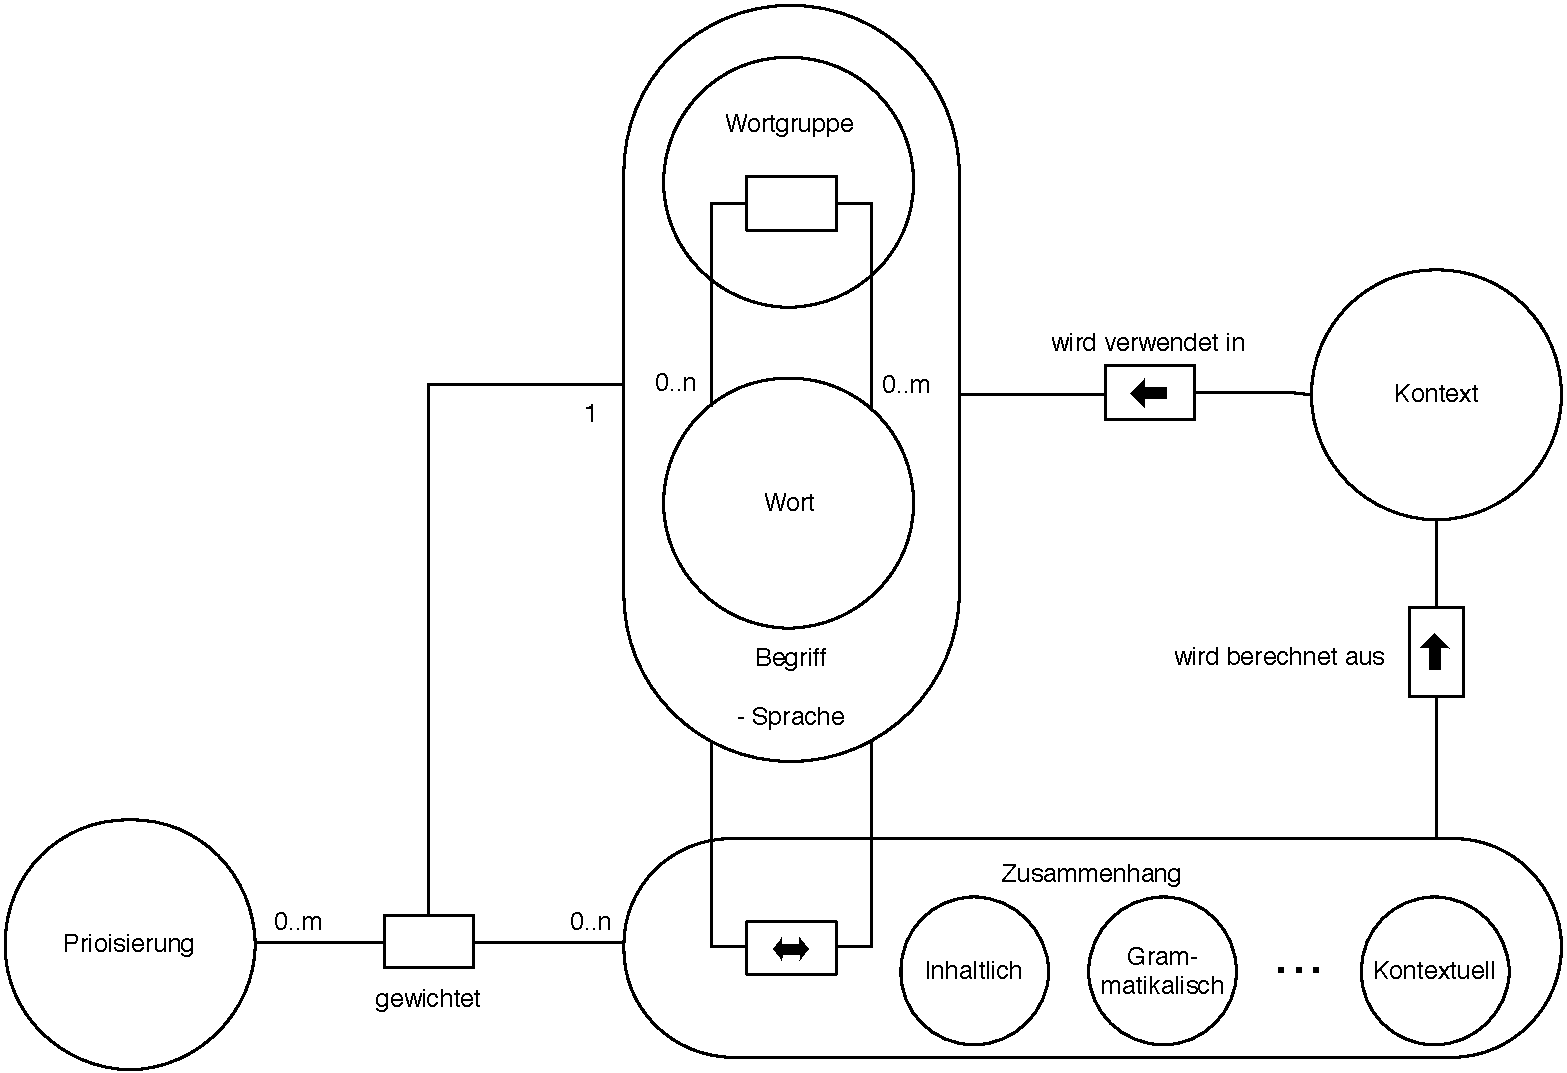
\includegraphics[width=\textwidth]{abstract_world_model}
\caption{FMC--Entity-Relationship--Diagramm des Modells des Weltausschnittes}
\label{fig:world_model}
\end{figure}

Abbildung \ref{fig:world_model} zeigt das Modell als Entity--Relationship--Diagramm.

Zentrale Entität ist des Modells der \emph{Begriff}. Ein Begriff repräsentiert ein Einzelwort oder eine Wortgruppe in einer bestimmten Sprache. Dies berücksichtigt den Umstand, dass Wörter in mehreren Sprachen vorkommen können, jedoch verschiedene Bedeutungen besitzen können. Wortgruppen können aus beliebig vielen Einzelwörtern zusammengesetzt sein. Mit Hilfe der Link Discovery sollen zwischen diesen Begriffen verschiedenartige \emph{Zusammenhänge} gefunden werden.

Ein Zusammenhang besteht immer zwischen genau zwei Begriffen und besitzt einen bestimmten \emph{Typ}. Der Typ bezeichnet die Art des Zusammenhangs zwischen diesen beiden Begriffen. Beispiele für Zusammenhangsarten sind inhaltliche Zusammenhänge wie Synonyme, grammatikalische Zusammenhänge wie Wortformen und Grundformen oder kontextuelle Zusammenhänge, die sich aus der Verwendung des Begriffes ergeben. Dabei kann ein Zusammenhang abhängig vom Typ Attribute besitzen, die den Zusammenhang genauer spezifizieren. Dies kann beispielsweise ein Gewicht des Zusammenhangs sein, dass die Wichtigkeit gegenüber anderen Beziehungen gleichen Typs angibt.

Je nach Nutzungsform der Daten wird unter Umständen eine andere Sicht auf die Beziehungen benötigt. Eine \emph{Prioisierung} stellt eine Gewichtung der Beziehungen eines Begriffes nach Typ dar. Sie teilt jeder Zusammenhangsart ein Gewicht relativ zu den anderen Arten zu. Somit werden durch die Prioisierung bestimmte Zusammenhänge höher gewichtet als andere. Die Prioisierung wird zu einer auf den Anwendungsfall abgestimmten Ordnung der Beziehungen eines Begriffes genutzt.

Dies Verwendung eines Begriffes wird durch den \emph{Kontext} beschrieben. Dieser Kontext repräsentiert, \emph{wo}, \emph{wie} und \emph{wann} der Begriff innerhalb einer bestimmten Anwendungsdomäne verwendet wurde. Daher sind die Attribute, die ein Kontext besitzen kann, nicht vorab spezifizierbar. Sie hängen von der jeweiligen Anwendungsdomäne ab. Beispiele für Kontexte sind die Verwendung eines Begriffes in einem Tag-System oder in einer Ontologie.

Dieses Modell bildet die Grundlage für  im folgenden Abschnitt beschriebenen Link--Discovery--Prozess.

\section{Link--Discovery--Prozess}
\label{ld_process}

Der Link--Discovery--Prozess beschreibt die Abfolge von Schritten, die zur Erzeugung und Anreicherung des in \ref{world_model} beschriebenen Weltausschnittes angewendet werden. Dieser Prozess dient also zur Erzeugung von Begriffen und deren Zusammenhängen. Abbildung \ref{fig:link_discovery_process} zeigt den Prozess als Petri--Netz.

\begin{figure}
\centering
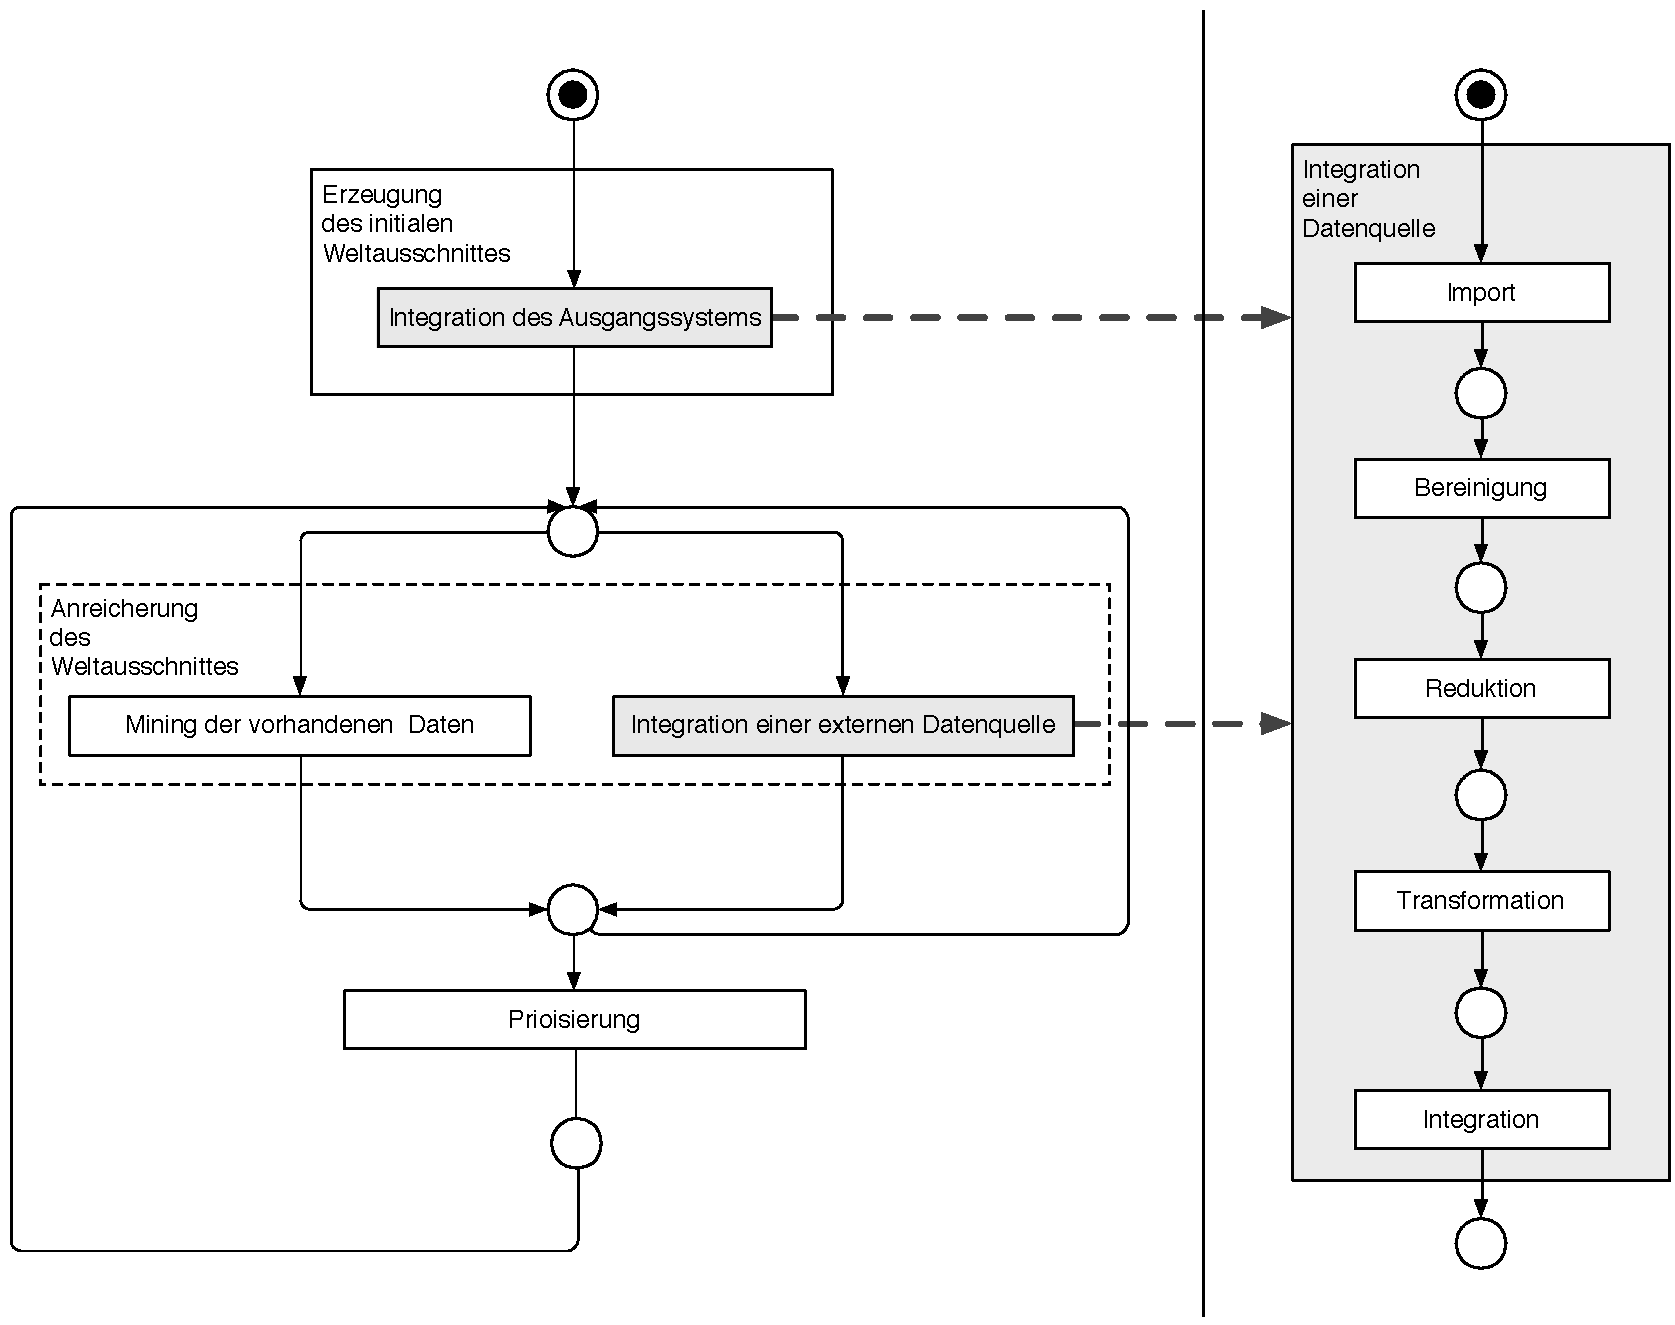
\includegraphics[width=\textwidth]{link_discovery_process}
\caption{FMC--Petri--Netz des Link--Discovery--Prozesses}
\label{fig:link_discovery_process}
\end{figure}

Die grundlegenden Phasen des Prozesses sind die \emph{Erzeugung} des initialen Weltausschnittes, dessen \emph{Anreicherung} und die \emph{Prioisierung} der Beziehungen. Sowohl bei der initialen Erzeugung, als auch bei der Anreicherung wird ein Prozess zur Integration von Datenquellen benötigt.

Die Schritte der Anreicherung und Prioisierung können beliebig oft wiederholt werden, um das Ergebnis zu verbessern und auf die gewünschte Anwendung anzupassen. Die Anreicherung kann grundsätzlich durch das Mining der bereits im Weltausschnitt vorhandenen Daten oder durch die Integration neuer Datenquellen erfolgen.

Die genannten Schritte werden in den folgenden Abschnitten erläutert.

\subsection{Integration von Datenquellen}
\label{integration_generic}

Für die Link Discovery wird ein einheitliches Vorgehen zur Integration von Datenquellen benötigt. Die Datenquellen stellen grundsätzlich für die Link Discovery nützliche Daten zur Verfügung, die jedoch im Allgemeinen noch nicht direkt dem Modell des Weltausschnittes entsprechen. Demzufolge müssen diese Daten entsprechend vorverarbeitet werden.

Die zur Integration von externen Datenquellen nötigen Schritte entsprechen im Wesentlichen den von \textcite[S. 48f.]{hkp2012} beschriebenen Aufgaben der Datenvorverarbeitung: \emph{Bereinigung}, \emph{Reduktion}, \emph{Transformation} und \emph{Integration}. Diesen wird in dieser Arbeit der Schritt \emph{Import} vorangestellt, da es nicht immer möglich ist, den gesamten Datenbestand einer Datenquelle zu nutzen. Somit sollten im Importschritt auch die Anfragen an die Datenquelle spezifiziert werden. Die genannten Schritte werden zur Link Discovery immer in der genannten Reihenfolge ausgeführt und werden im folgenden kurz beschrieben.

\paragraph{Import}

Im Importschritt werden die Rohdaten aus der Datenquelle extrahiert. Dabei wird die Form der Daten nicht verändert. Ist es nicht möglich, den gesamten Datenbestand einer Quelle zu importieren, so muss eine Auswahl der anzufragenden Daten formuliert werden. Diese Auswahl richtet sich nach Möglichkeit nach den bereits im Weltausschnitt vorhandenen Daten.

\paragraph{Bereinigung}

Im nachfolgenden Bereinigungsschritt werden die importierten Daten so gut wie möglich von eventuell vorhandenen Defekten bezüglich der Datenqualität (siehe auch \ref{quality}) befreit. Dazu zählen beispielsweise das Entfernen nicht nutzbarer Zeichen oder von unvollständigen Datensätzen.

\paragraph{Reduktion}

Der Reduktionsschritt dient zur Verkleinerung der Datenmenge. Dazu gehören beispielsweise Schritte zur Duplikatentfernung oder zur Auswahl relevanter Datensätze. In dieser Arbeit bestand die Haupteinschränkung der Datenmenge darin, nach Möglichkeit nur deutschsprachige Datensätze auszuwählen.

\paragraph{Transformation}

Der Schritt der Transformation überführt die Daten schließlich in das Modell des Weltausschnittes. Dies bedeutet, dass die Datensätze in Begriffe und Beziehungen umgewandelt werden. Dabei sollten so viele Informationen über den Kontext der Begriffe erhalten bleiben. Die Methode, wie diese Transformation vorgenommen wird, hängt von der Datenquelle ab. Generell werden die Beziehungen meist aus dem Kontext der Begriffe, wie er in der Datenquelle vorliegt, gebildet. Somit stellt der Transformationsschritt die wichtigste Komponente für die Integration einer Datenquelle dar.

\paragraph{Integration}

Der Integrationsschritt für jede Datenquelle dient letztendlich der Zusammenführung des im Transformationsschritt erzeugten Weltausschnittes mit dem bereits vorhandenen Weltausschnitt. Dabei werden bereits existierende Begriffe zusammengeführt und die neu erzeugten Beziehungen übernommen. Die Zusammenführung der Begriffe erfolgt über die Annotation des existierenden Begriffes mit dem neu erzeugten Kontext, den die Datenquelle zu einem Begriff liefert.

\subsection{Initiale Erzeugung des Weltausschnittes}

Der erste Schritt der Link Discovery besteht in der Auswahl einer geeigneten Datenquelle für die initiale Erzeugung des Weltausschnittes. In dieser Arbeit ist diese Datenquelle das Tagging-System von Spreadshirt (siehe \ref{tag_sprd}).

Die Auswahl der Datenquelle richtet sich im wesentlichen danach, ob der Kontext, den die Datenquelle potentiell zu Begriffen liefern kann, für die Link Discovery geeignet ist. Der Kontext sollte außerdem für die geplante Anwendung der Link--Discovery--Ergebnisse relevant sein.

Nach der Auswahl einer geeigneten Quelle werden die in Abschnitt \ref{integration_generic} beschriebenen Schritte zur Integration durchgeführt. Der letzte Schritt ist trivial, da zu diesem Zeitpunkt noch keine Daten im Weltausschnitt vorhanden sind.

\subsection{Anreicherung des Weltausschnittes}

Nach der initialen Erzeugung des Weltausschnittes kann dieser mit beliebig vielen Anreicherungsschritten ergänzt werden. Unter Anreicherung wird die Erzeugung neuer Begriffe, Kontexte oder Zusammenhänge verstanden.

Das Hinzufügen neuer Begriffe erweitert das Vokabular des Weltausschnittes. Somit können bei der Benutzung der Daten zu einer größeren Menge von Begriffen Zusammenhänge gefunden werden. Die Erzeugung von Kontexten zu vorhandenen oder neuen Begriffen erweitert das Wissen über die Benutzung eines Begriffes innerhalb einer bestimmten Anwendungsdomäne. Die Anreicherung des Weltausschnittes mit neuen Zusammenhängen ermöglicht einerseits das Finden von relevanten Nachbarn eines Begriffes, erfordert andererseits jedoch, abhängig von der Anwendung, auch eine andere Prioisierung der Zusammenhangstypen bei der Abfrage.

Grundsätzlich kann die Anreicherung des Weltausschnittes auf zwei Arten erfolgen. Dies ist zum die Anreicherung durch das Mining der bereits vorhandenen Daten, zum anderen die Anreicherung durch Integration einer weiteren Datenquelle.

\subsubsection{Anreicherung durch Mining vorhandener Daten}

Die Erzeugung neuer Begriffe und Zusammenhänge kann aus den vorhandenen Daten mittels Methoden des Data Minings vorgenommen werden. Dazu werden die bereits im Weltausschnitt vorhandenen Begriffe mit ihren Kontexten und Beziehungen analysiert, um bisher unbekannte Zusammenhänge zu finden.

Beispiele für anwendbare Methoden sind hierbei Assoziationsanalyse \cite[S. 328f.]{pt2013} oder Clusteranalyse \cite[S. 443f.]{hkp2012}, um bestimmte bereits in den Daten vorhandene, aber nicht explizit abgebildete, Zusammenhänge zu ermitteln. Jedoch können auch einfachere Methoden wie die Zerlegung von Wortgruppen in Einzelwörter (siehe \ref{decomposition}) erfolgreich sein, um neue Begriffe und Beziehungen in den Datenbestand einzuführen.

\subsubsection{Anreicherung durch Integration externer Datenquellen}

Sofern weitere Datenquellen verfügbar sind, stellt die Integration dieser einen weiteren erfolgversprechenden Weg dar, um die Daten anzureichern. Neue Datenquellen beschreiben immer einen neuen Kontext, in dem Begriffe genutzt werden. Ist der Kontext dieser Begriffe für die spätere Anwendung relevant, ist die Integration der jeweiligen Datenquelle zu Zwecken der Link Discovery von großem Interesse.

Um die zusätzliche Datenquelle zur Link Discovery zu nutzen, werden die gleichen Schritte, die schon zur initialen Erzeugung des Weltausschnittes zum Einsatz kamen, genutzt (siehe \ref{integration_generic}). Dazu werden im Transformationsschritt Daten erzeugt, die dem Modell des Weltausschnittes entsprechen. Im Integrationsschritt werden sie mit den bereits vorhandenen Daten zusammengeführt.

\subsection{Prioisierung von Beziehungen}